
\section{Introduction}
    Instruction reordering is a common operation done by the compiler / hardware for optimization, essential to instruction scheduling of course, but also implicit in loop invariant removal, partial redundancy elimination, and other optimizations that may move instructions. 
    However, whether we can do such reordering freely given a concurrent program using relaxed memory accesses is a bit unclear. 
     
    \paragraph{Simple reordering is not straightforward under shared memory semantics}
    The main reason is that memory accesses here, do not just perform the desired operation (i.e Read / Write) but also imply certain visibility guarantees across all the other threads.  
    In our observation, we find that, the relaxed memory model of Javascript prescribe semantics for visibility using the $\stck{_{hb}}$ relations. 
    
    \paragraph{Some Examples}

        We show a couple of examples to showcase why reordering may not be that straightforward. 

        Consider the first example below of a Candidate and the resultant candidate after reordering two events:
        
        %Put figure here
        \begin{figure}[H]
            \centering
            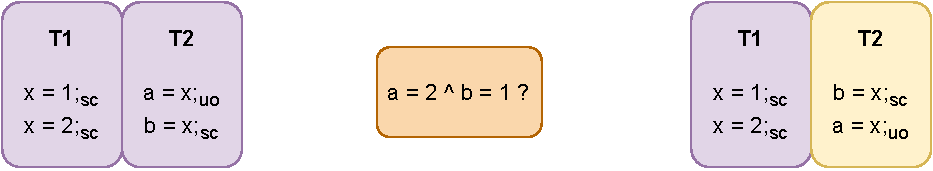
\includegraphics[scale=0.7]{5.InstructionReordering/ReorderingExample1(a).pdf}
            \caption{Ex1(a)} 
        \end{figure}

        The figure on the left is the original candidate and that on the right is after reordering the two reads of $T2$.
        The observable behavior in question is written in the middle. 

        %Put figure of explaination below
        \begin{figure}[H]
            \centering
            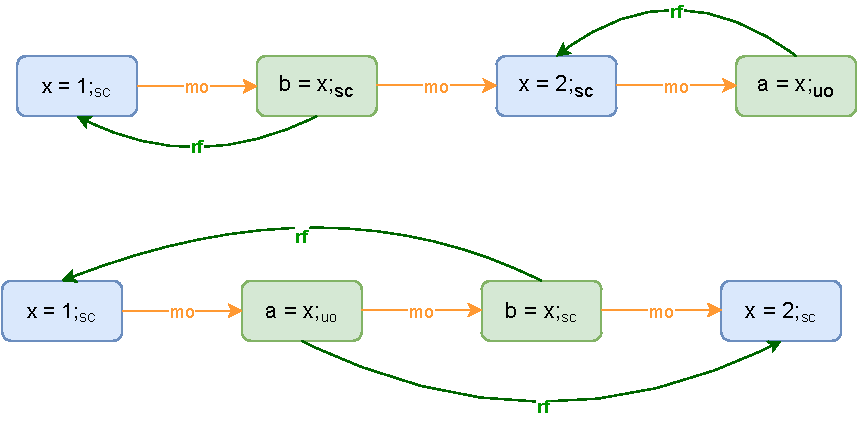
\includegraphics[scale=0.7]{5.InstructionReordering/ReorderingExample1(b).pdf}
            \caption{Ex1(b)} 
        \end{figure}

        The above figure has two sets of relations. The first justifies the outcome for the reordered candidate. While the second justifies the first. 
        Notice that for the second, one may have a read memory ordered before a write that it reads from. 
        This is quite counter intuitive to understand at first. 
        But strictly from the semantics of the model, this justification of the observable behavior is completely valid. 

        Consider another example below:

        %Put figure here 
        \begin{figure}[H]
            \centering
            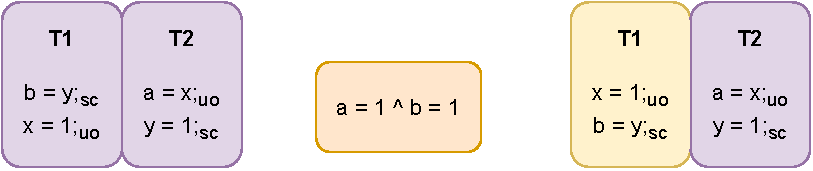
\includegraphics[scale=0.7]{5.InstructionReordering/ReorderingExample2(a).pdf}
            \caption{Ex2(a)} 
        \end{figure}

        The figure on the left is the original candidate and that on the right is after reordering the two events of $T1$.
        The observable behavior in question is written in the middle. 

        %Put figure here
        \begin{figure}[H]
            \centering
            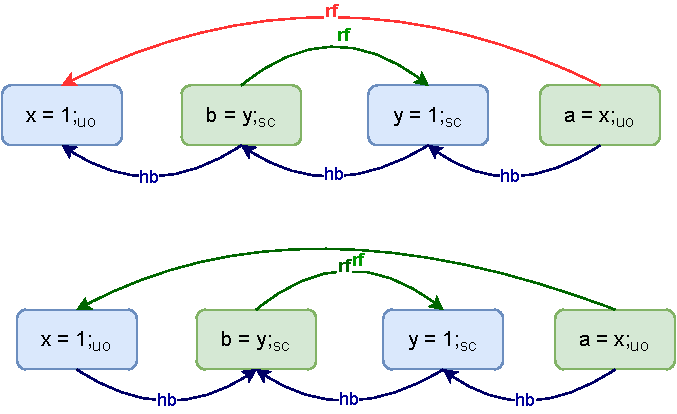
\includegraphics[scale=0.7]{5.InstructionReordering/ReorderingExample2(b).pdf}
            \caption{Ex2(b)} 
        \end{figure}

        The above figure has two sets of relations. The first justifies that such an outcome is not possible for the original program candidate due to Axiom \ref{CoRe}. While the second justifies that this outcome is possible for the reordered program.
        
        Note that we cannnot infer in the reordered candidate the set of relations for any candidate execution to have $\reln{a=x;_{uo}}{hb}{x=1;_{uo}}$. 

        The point of the above two examples is to show that we have to be careful while reordering two events in the same thread. By example case analysis, for each observable behavior, one must check all possible candidate executions and assert whether such an observable is possible or not. 
        This method of checking validity of reordering will scale exponentially as the program size increases. 
        It is often also the case that the compiler may not have information on which exact events would be executed in other threads to assert such reordering is valid or not. 

    
    
    
    
    